\chapter{List-based Query Processing}
\label{list-based-processing}

In this chapter, we introduce a new query processing technique, List-based query processing, for executing queries in a \gls{gdbms}. Our new processing technique benefits from orederly access of edges and its properties from the adjacency lists and edge property lists. Section~\ref{sec:existing-techniques} describes the different query execution models and lists the pros and cons for each of them. Next, we describe List-based processing in Section~\ref{sec:list-based-proc}

\section{Existing Techniques}
\label{sec:existing-techniques}
Almost all the \gls{gdbms} we are aware of uses the \textbf{Volcano-styled iteration model}~\cite{volcano} to execute a query. In the volcano-styled execution pipeline, each operator stores the reference of the next operators in the query plan. Execution happens tuple-at-a-time, with either operator operating on a partial match and pushing the result to the new operator in the pipeline. In particular, while processing a query volcano-styled, the edges of an adjacency list is read one at a time and processed further, making the access to the edge essentially random. Thus, this technique is oblivious to the fact that the edges in the adjacency lists are read in the same order in which they are stored, as stated in our Guideline~\ref{ssec:edges-ordered}. Clearly, processing the query volcano-styled does not agree with our Desiridatum~\ref{des1}. Even for the case of reading edge properties, we do not derive cache locality benefits from storing the properties of sequential edges nearby, since the access is mostly random. Also, the number of operations that are executed with volcano-styled processing is very high owing to the fact that each operator is particularly called as many times as there are input partial matches to. The large number of function calls adds significantly to the runtime of query execution on rad-intensive workloads.

\begin{example}
	\vspace{5pt}
	\label{ex:proc-example}
	Consider the following query. 
	{\em 
		\begin{lstlisting}[numbers=none,  showstringspaces=false,belowskip=0pt ]
		MATCH (a:PERSON)$-$[ex:FOLLOWS]$\rightarrow$(b:PERSON),
		$\qquad\quad$(b:PERSON)$-$[ey:FOLLOWS]$\rightarrow$(c:PERSON)
		WHERE a = $v4$
		RETURN ey.since\end{lstlisting}
	}
\end{example}
\vspace{-5pt}

\begin{figure}
	\hfill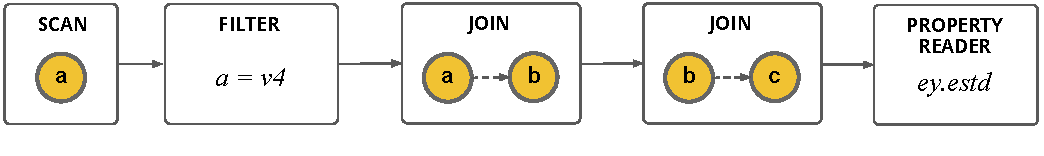
\includegraphics[scale=0.78]{img/proc-qp}\hfill
	\vspace{-10pt}
	\caption{Query plan for Example~\ref{ex:proc-example}.}
	\vspace{-8pt}
	\label{fig:proc-qp}
\end{figure}

Example~\ref{ex:proc-example} shows a 2-hop query starting from $v4$ of our example graph, while Figure~\ref{fig:proc-qp} shows a plan to execute the 2-hop query. In a volcano-styled processing-based system, this query is matches $a$ to $v4$ and $ex$ and $b$ respectively to the first element in $v4$'s adjacency list, i.e, $e2$ and $v1$. Next, $ey$ and $c$ is matched to the first edge in $v2$'s adjacency list, i.e. $e1$ and $v2$, before reading $e1$'s \texttt{since} property. Then, $ey$ is matched to $e9$ ($v2$'s second edge) and its property is returned. Now since $v2$'s adjacency list is exhausted, $ex$ is matched to second edge in $v4$'s adjacency list and processing continues. 

Alternative to volcano-styled iterator model is \textbf{column-at-a-time processing}~\cite{boncz-phd, monet-2decades} that is prevalent with columnar stors. While processing a column, this technique employs efficient block algorithms and tight loop over arrays that draw benefits from advanced compiler optimizations and even SIMD instructions in modern CPUs. Column-at-a-time processing can be applied to execute queries in \gls{gdbms}, in general, and to our solution, in particular, where it benefits from reading edges and its properties sequentially. The downside of operating column-at-a-time is the enormous amount of intermediary data that is produces with each operator that limits the execution in scalibility. This drawback is alleviated by yet another technique, called \textbf{Vectorized processing}~\cite{boncz-vectorwise1, boncz-monet-vectorized, boncz-vectorwise, dbms-cache}, that proceses vector-at-a-time. Vectorized processing sits in beween the above two solution as it combines volcono-styled pipelineing with processing techniques of column-at-a-time processing. 

An intrinsic problem with operating vector-at-a-time or column-at-a-time is that of data duplication. The values of a vector gets duplicated each time an already matched vertex $v$ gets joined to an edge in $v$'s adjacency list. Hence, the duplication in query execution amplifies with each subsequent \texttt{JOIN}s in a query plan. Executing the query plan in Figure~\ref{fig:proc-qp} on example graph, the output of \texttt{SCAN(a)} is a single element vector $[v4]$. When \texttt{JOIN}ed with $b$, output is $[v4, e2, v1]$, $[v4, e5, v2], [v4, e3, v5]$, with $v4$ repeated in each. Joining with $c$ requires further duplication of $v4$ and its adjacent edges.

\section{List-based Processing}
\label{sec:list-based-proc}

A typical workload on a \gls{gdbms} involves matching long path queries on the input graph, which means a large number of usage of \texttt{JOIN} operators in the query plan. If such a query is executed in vectorized processing model, the problem of data duplication gets aggrevated to extreme levels and bulk of the query execution time is wasted in copying the input partial match. On the other hand, using pure volcano-style processing do not reap the benefits of ordered arrangement of data in adjacency lists and property pages. To elevate the problem of data duplication, we present a new query execution technique called \textbf{List-based processing}, that still uses the volcano-styles nesting of operators but processes a query by one adjacency list-at-a-time. In particular, a vertex $v$ in the partial match is joined to edges and neighbour vertices in $v$'s adjacency list in a single execution of \texttt{JOIN} operator. Moreover, the result of the join is processed in a single operation by other operators like \texttt{PROPERTY READER} and \texttt{FILTER}.















